\documentclass[11pt]{report}
\usepackage[utf8]{inputenc}
\usepackage[danish]{babel}
\usepackage [T1]{fontenc}
\usepackage[margin=2.5cm]{geometry}
\usepackage[hidelinks]{hyperref}
\usepackage{graphicx}
\graphicspath{{img/}}
\usepackage{listings}
\usepackage{color}
\usepackage{adjustbox}
\usepackage{tocloft}
\usepackage{listings}
\usepackage{enumitem}
\usepackage{indentfirst}
\usepackage{caption}
\usepackage{float}
\usepackage{titlesec}
\usepackage{fancyhdr}
\usepackage{lastpage}
\titleformat{\chapter}[display]   
{\normalfont\huge\bfseries}{\chaptertitlename\ \thechapter}{20pt}{\Huge}
\titlespacing*{\chapter}{0pt}{-30pt}{40pt}

\setlength{\parskip}{12pt}

\definecolor{dkgreen}{rgb}{0,0.6,0}
\definecolor{gray}{rgb}{0.5,0.5,0.5}
\definecolor{mauve}{rgb}{0.58,0,0.82}

\lstset{frame=tb,
  language=Java,
  aboveskip=3mm,
  belowskip=3mm,
  showstringspaces=false,
  columns=flexible,
  basicstyle={\small\ttfamily},
  numbers=none,
  numberstyle=\tiny\color{gray},
  keywordstyle=\color{blue},
  commentstyle=\color{dkgreen},
  stringstyle=\color{mauve},
  breaklines=true,
  breakatwhitespace=true,
  tabsize=3
}

\definecolor{bluekeywords}{rgb}{0.13,0.13,1}
\definecolor{greencomments}{rgb}{0,0.5,0}
\definecolor{turqusnumbers}{rgb}{0.17,0.57,0.69}
\definecolor{redstrings}{rgb}{0.5,0,0}


\lstdefinelanguage{FSharp}
                {morekeywords={let, new, match, with, rec, open, module, namespace, type, of, member, and, for, in, do, begin, end, fun, function, try, mutable, if, then, else},
    keywordstyle=\color{bluekeywords},
    sensitive=false,
    morecomment=[l][\color{greencomments}]{///},
    morecomment=[l][\color{greencomments}]{//},
    morecomment=[s][\color{greencomments}]{{(*}{*)}},
    morestring=[b]",
    stringstyle=\color{redstrings}
    }
\usepackage{amsmath}
\makeatletter
\let\ps@plain\ps@fancy
\makeatother
\pagestyle{fancy}
\fancyhf{}
\fancyhead[L]{Asger Hermind Sørensen}
\fancyhead[C]{Praktikrapport}
\fancyhead[R]{23. oktober 2020}
\fancyfoot[R]{Side \thepage\ af \pageref*{LastPage}} 
\renewcommand{\headrulewidth}{1pt}

\begin{document}
\begin{titlepage}
  \begin{center}
      \vspace*{1cm}

      \Huge
      \textbf{Praktikrapport 2020}

      \vspace{0.5cm}
      \LARGE
      Hos Efio ApS

      \vspace{1.5cm}

      \textbf{
        Asger Hermind Sørensen\\
        \texttt{cph-as466@cphbusiness.dk}
      }

      \vfill

      Praktikrapport for Datamatiker 5. Semester

      \vspace{0.8cm}

      \Large
      Datamatiker\\
      Cphbusiness Lyngby\\
      Danmark\\
      23. oktober 2020

  \end{center}
\end{titlepage}
\renewcommand{\cftchapleader}{\cftdotfill{\cftdotsep}}
\tableofcontents
\newpage

\chapter*{1. Fordord}
\addcontentsline{toc}{chapter}{1. Fordord}
Denne rapport er skrevet ud fra mit praktikophold i Efio ApS hovedkontor i København. 
Jeg har arbejdet gennemsnitligt 35 timer om ugen både på Efio’s kontorer samt hjemmefra.

Rapporten tager udgangspunkt fra praktikkens start den 17. august 2020 frem til den 21. oktober 2020.

Praktikopholdet har været i gruppe sammen med Andreas Zoega Vestergaard Vikke og Martin Eli Frederiksen. 

Efio har brug for et timeregistreringssystem for de kunder som de er ude hos. Konsulenterne glemmer at få registreret timerne korrekt, og det estimeres at der kan gå op til 100.000 kr. i tab over manglende registrerede timer. Dette grunder i at Efio fakturerer per påbegyndte halve time, og de skal huske minuttet de begyndte og minuttet de stoppede.
Systemet skal ligge som en applikation på kommunikationsplatformen Slack. 
 
 

\chapter*{2. Beskrivelse af praktikvirksomheden}
\addcontentsline{toc}{chapter}{2. Beskrivelse af praktikvirksomheden}
Efio er et konsulentfirma, som specialiserer sig i DevOps. DevOps specialisere sig i automation, infrastruktur som kode, serverless first nano services og continuous integration and delivery. Alt dette kan de tilbyde i Cloud Computing form og har store kunder såsom DR, Danmarks National Bank, Coop, Novo og mange flere.
Efio er et AWS Partner selskab hvilket vil sige de udbyder deres services på AWS platformen. De er omkring ca. 6 ansatte som Senior DevOps konsulenter, og har med os 5 praktikanter.

\chapter*{3. Hvordan jeg har opfyldt mine læringsmål}
\addcontentsline{toc}{chapter}{3. Hvordan jeg har opfyldt mine læringsmål}

\section*{3.1 viden}
\addcontentsline{toc}{section}{3.1 viden}
Efio har to afdelinger, en i København og en i Odense. De har også endnu et praktikhold i Odense ud over os. 
Efio arbejder som konsulenter ude hos de virksomheder som de har som kunder, og er derved sjældent på egne kontorer. 
Hvad kunden har behov for kan variere meget, og derved også konsulentens arbejde. 
De fleste konsulenter har en fast kunde de er ude hos, og arbejder projektvis hos en kunde. 

Efio har 4 kunde segmenter , de store virksomheder i lange ophold er det som Efios konsulenter hovedsageligt foretager sig. 
Men nogle små virksomheder kan også have brug for hjælp til at få ordnet fejl som kunden ikke kan eller ved hvordan skal ordnes. 
Små virksomheder kan også købe klippekort til Efios konsulenter.

Efio laver et daily stand-up på slack, så alle løbende ved, hvad hinanden arbejder på, 
selvom de ikke ser hinanden eller arbejder sammen i en længere periode. 
Dette bliver man påmindet om dagligt fra en bot, som også antyder hvordan det skal skrives, som kan ses på billedet forneden.
\begin{center}
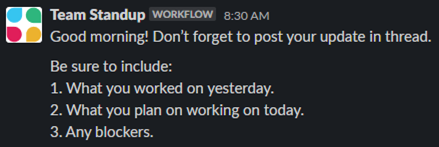
\includegraphics{standup}
\end{center}

\section*{3.2 Læringsmål}
\addcontentsline{toc}{section}{3.2 Læringsmål}
\subsection*{Problemløsning og Problemudvikling}
Joachim, direktør for Efio og vores tutor, har været inde over hele udviklingsprocessen, 
og har været med til at tænke kritisk og logistisk på en praksisorienteret måde. 
Joachin har gået meget op i, at vi følger scrum helt rigtigt, og at vi inddrager dens elementer. 
Joachim startede sprintsne med at redegøre for hvad der skulle laves, og gjorde rede for, hvordan det skulle udføres og kobles sammen. 
Det har derefter været vores opgave at prøve at udføre det, og hvis der opstod nogle problemer, 
diskuterede vi det internt eller talte med Joachim til stand-up mødet vi normalt har om eftermiddagen. 
Jeg har stødt ind i flere problemer, som jeg har skullet formidle til Joachim, hvor vi sammen har fundet en løsning, som han synes passer bedst. 

Vi har snakket sammen med Joachim om arkitektur på backenden af systemet. Her blev hele tankegangen af hvordan systemet diskuteret og udviklet. 
På det første billede er der det sidste udkast af hvordan backenden skulle fungere. Renskrevet version kan findes ved bilag x.
\begin{center}
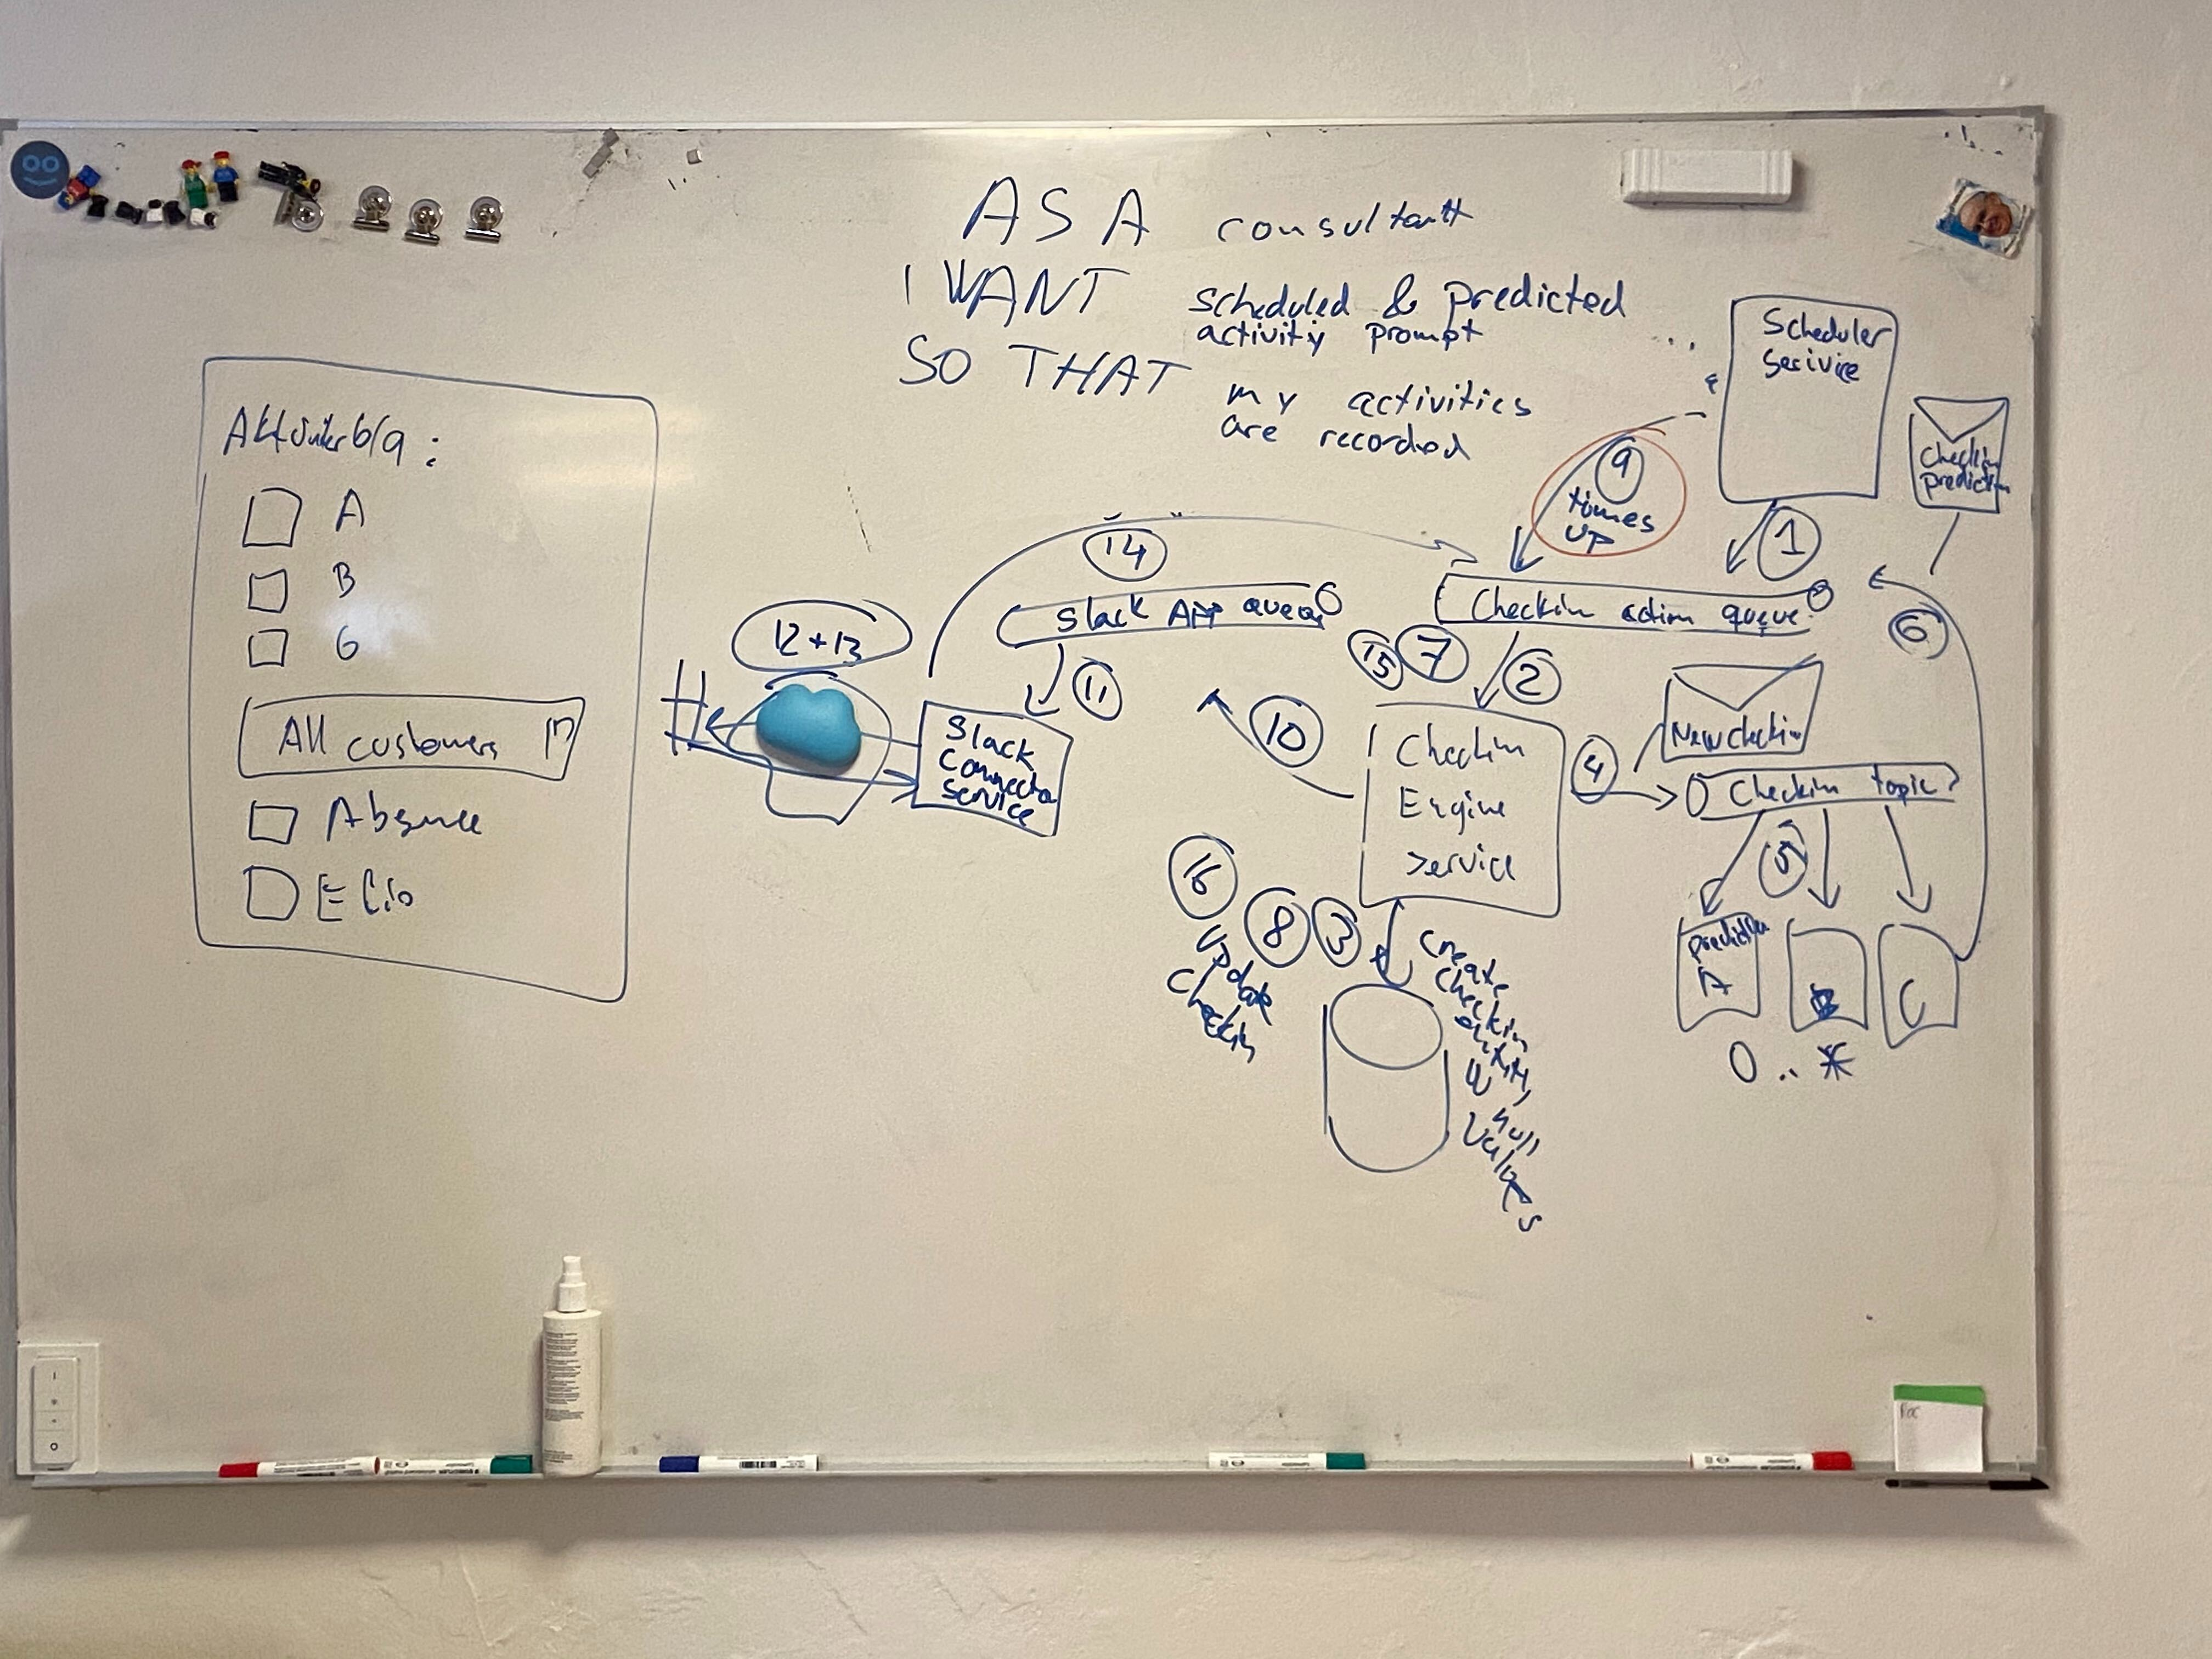
\includegraphics[height=11.93cm, width=15.9cm]{struktur}
\end{center}


\subsection*{Tekniske og Analytiske Arbejdsmetoder}
Vi har brugt rigtig meget scrum til udviklingen af det produkt vi sidder med. 
Jeg har kendskab til, eller har hørt om alt det vi har arbejdet med. 
Der blev sat meget fokus på definition of ready og definition of done, som jeg kun kort har hørt om på skolen.
Definition of ready består af INVEST:

\begin{itemize}
  \item Independent
  \item Negotiable
  \item Valuable
  \item Estimable
  \item Small
  \item Testable
\end{itemize}

For at en user story er klar til at kunne blive sat i sprint backlog, skal den opfylde INVEST. 
Det kræver at userstoryen:

\begin{itemize}
  \item Er uafhængig af andre user storys.
  \item Kan ændres og diskuteres, det er ikke en kontrakt for en feature.
  \item Bringer en form for værdi, enten til systemet, brugerne eller aktionere. 
  \item Kan rimeligt estimeres.
  \item Ikke er for stor til ikke at kunne passe i et sprint.
  \item Kan testes, og kræve nok information til at der kan laves test driven development eller behaviour driven development
\end{itemize}

Hvis en user story kan opfylde alle de krav kan den derved tages med i sprintet. 
Da vi kørte dette projekt, skulle alle være enige om hvert punkt i INVEST var opnået før definition of ready var opfyldt. 
Hvis ikke diskuterede vi for og imod punktet, og lavede ændringer hvis nødvendigt. 

Når en user story er klar til at blive gennemgået, og skal lægges over som færdig, skal den først kunne opnå definition of done:

Definition of Done:

\begin{enumerate}
  \item automatiseret godkendelse af acceptens kriterier
  \item gennemgået af holdmakker(e)
  \item fusioneret med master
  \item Deployere til produktion
\end{enumerate} 

Første punkt bliver kørt igennem Cucumber’s Behave, som kører accept test i python som en del af Behaviour Driven Development (BDD). 
Der testes lokalt før man pusher op, men alle behave test køres automatisk oppe på CI-pipelinen når man pusher op på en feature branch. 

Der kan ikke merges ind til master uden at man laver et pull request. 
Dette pull request kræver at en anden fra ens hold gennemgår ens kode, og tjekker, at det man har lavet er i orden 
og at koden opnår en vis kvalitet. Derved får man klaret punkt 2 og 3 ved pull requestet. 
Når en holdmakker godkender ens pull request kan man merge ind til master.

Til sidst opretter man en ny udgivelse på GitHub, det er CD pipeline sat op til at lytte efter. 
Når en ny udgivelse er lavet, sender GitHub et request til pipelinen om at der er lavet en ny release som CD-pipelinen lytter på. 
Så går den i gang med at bearbejde. Når pipelinen er kørt igennem og alt fungerer, er der blevet deployeret til produktion. 


\subsection*{Struktur}
Vi har brugt Jira til at opstille struktur omkring den individuelle arbejdsgang. 
Jira er en platform der bruges til agile udviklingsmetoder. Jira har hele vores sprint backlog, hvor hver user story er brudt ned i subtasks. 

Alle user storys kommer fra sprint planning meeting med PO, hvor vi sammen har siddet og bedømt hvor mange user storys 
vi kan tage på et sprint, med henhold til den viden vi besidder på nuværende tidspunkt. 
For at kunne bedømme hvor stor en user story er, har vi brugt poker planning sammen med risk evaluation, 
for at kunne bedømme om den størrelse der er givet til user story har en lille eller stor chance for at ramme forkert. 
Risk evaluation bliver baseret på hvor meget vi kender til de teknologier som user storyen indebærer. 

Hver dag har vi en daily stand-up, og taler med hinanden om, hvad vi arbejder på, og om vi har nogle problemer vi eventuelt 
har brug for noget hjælp til. Derved har vi altid et overblik over hvor hele holdet er henne. 
Hvis der ikke er nogen der har brug for hjælp, har vi arbejdet individuelt videre på den user story man er på, 
eller tilknytter sig en ny user story eller subtask. 


\section*{2.3 Kompetencer}
\addcontentsline{toc}{section}{2.3 Kompetencer}

\subsection*{Tilegnelse af ny viden}
De første tre uger gik næsten kun ud på at tilegne sig viden omkring serverless computing, 
AWS og deres tjenester. Meget af det har været svært at forstå, da det er noget helt andet 
end det vi har arbejdet med på skolen. Selve brugen af tjenesterne har ikke været utroligt svært, 
men forståelsen af hvordan de forskellige tjenester fungerer har været det jeg har haft meget svært med. 
Joachim har gennemgået mange af de ting som jeg har fundet svært, og virkelig gået i dybde med de forskellige 
systemer og tjenester som vi har taget i brug så jeg kan få en dybere forståelse. 

\subsection*{Faglig og tværfaglig}
Jeg har hovedsageligt gjort brug af systemudvikling med scrum. 
Her har vi også haft Peter inde over, som er virkelig god til at se problematikker for brugeroplevelsen. 
Her har vi snakket sammen om, hvordan vi kunne forbedre designet af vores produkt, for at gøre det mere brugervenligt. 

Herefter har vi også haft et møde med den anden praktik gruppe i Odense, 
for at høre om hvad de lavede, samt få deres input til hvordan vi kunne forbedre vores eget produkt.


\chapter*{3. Udførte arbejdsopgaver}
\addcontentsline{toc}{chapter}{3. Udførte arbejdsopgaver}
\subsection*{sprint 0}
Før der kunne begyndes på projektet, var jeg nødt til at lærer omkring AWS og de tjenester som de tilbyder. 
Dette indeholder bl.a. at få et certifikat fra Amazon om gennemførelse som AWS Techical ProfessionalFOOTNOTE HERE. 
Herudover brugte jeg lang tid på at få online undervisning omkring AWS og deres tjenester samt hvordan man bruger dem igennem a cloud guruFOOTNOTE HERE.

\subsection*{sprint 1}
\begin{center} 
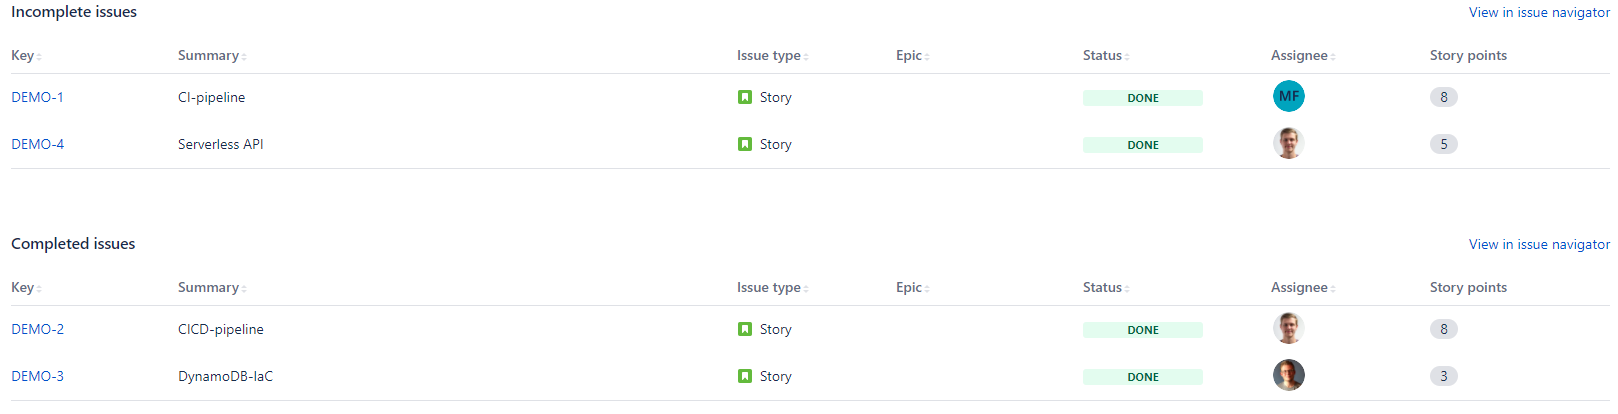
\includegraphics[height=4.13cm, width=15.92cm]{sprint1}
\end{center}

I projektets første sprint startede jeg med at opbygge en NoSQL database, DynamoDB. 
Jeg har efterhånden skulle opbygge en del databaser med relationer, men logikken er helt anderledes. 
Det er ikke noget vi har lært på skolen, men har heller ikke været anset nødvendigt. 
Resten af gruppen har opbygget Continuous Integration (CI) og Continuous Deployment (CD) pipelines. 
Det har vi kun fået en dags undervisning i. Derved var det svært at forstå hvordan det fungerede til at starte med, 
og siden jeg ikke selv har bygget den, er min viden om den stadig begrænset.  

\subsection*{sprint 2}
\begin{center} 
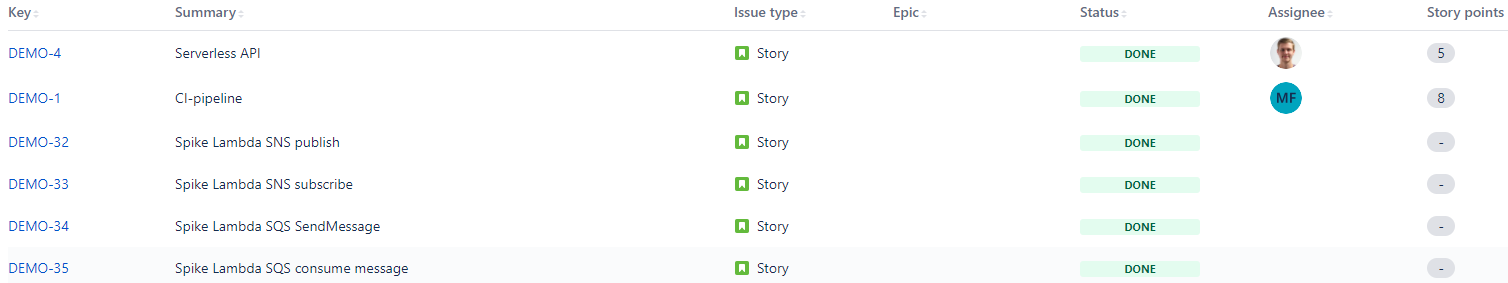
\includegraphics[height=4.13cm, width=15.92cm]{sprint2}
\end{center}

Idet der blev arbejdet på meget nye tjenester, blev andet sprint sat af til Spikes. 
Spikesne omfatter brugen af lambda funktioner, som er en begivenhedsdrevet serverløs computing platform, 
så man kan køre kode uden at skulle håndtere servere.

En af de lambdafunktioner skal kunne skrive til en Simple Queue Service (SQS), 
som holder beskeder i kø som derefter kan køres af andre lambdafunktioner. 
Der skulle dertil også en lambdafunktion til at kunne tage en besked fra SQS-køen og gøre noget ved den besked.

En anden lambdafunktion skulle kunne skrive fra en Simple Notification Service (SNS), 
som kan skrive beskeder, e-mails, SMS mm. ud til alle som abonnere på et emne som den SNS omhandler. 
Man kan bruge en lambdafunktion til at skrive beskeder ud fra SNS, som derved bliver sendt ud til alle der abonnerer, 
hvilke kan være en anden lambdafunktion som gør noget ved den besked. 


\subsection*{sprint 3}
\begin{center} 
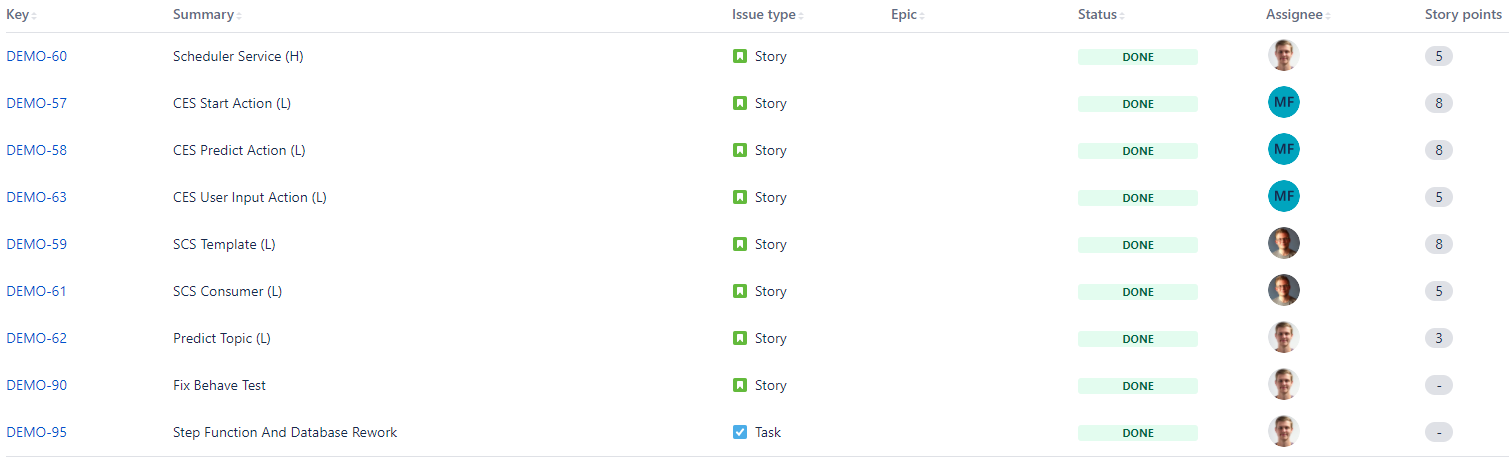
\includegraphics[height=4.13cm, width=15.92cm]{sprint3}
\end{center}

Her havde jeg fokus på Slack Connection Service (SCS), som er at snakke med Slacks API igennem den app vi havde lavet. 
Det bestod af at kunne sende en knap til en kanal i Slack, som en bruger kan trykke på. Her brugte jeg meget postman 
for at finde ud af hvordan Slacks API fungerede, som vi har brugt meget i skolen. 

Når brugeren trykker på knappen, skal der poppe et Modal op. Modalet blev designet sammen med PO under sprint planning. 
Modalet skulle udfyldes med de kunder som brugeren kunne have været ud hos, som var blevet forudsagt og ligger i 
databasen. Inden modalet bliver sendt til brugeren skal modalets template blive udfyldt med det data der ligger i 
databasen. Modalets template er bygget i JSON, og kunne derved nemt manipuleres med andet data. Jeg kender til brug 
af API og manipulation af JSON fra skolen af, og var derved ikke en større udfordring. 

\subsection*{sprint 4}
\begin{center} 
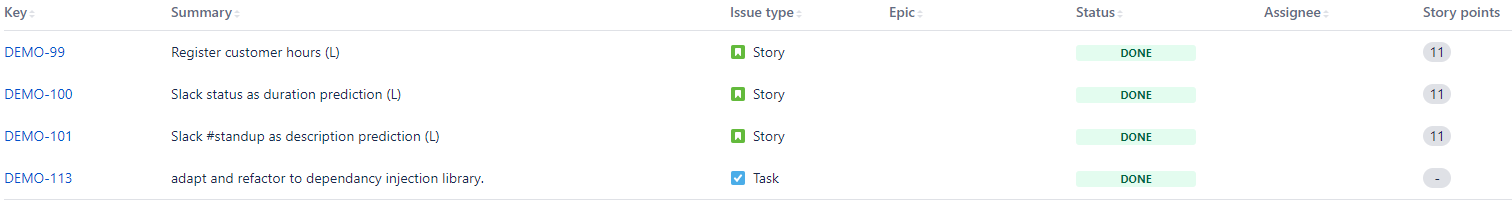
\includegraphics[height=4.13cm, width=15.92cm]{sprint4}
\end{center}

Joachim ville gerne have ændret måden data blev gemt på i databasen når en bruger valgte en kunde i modalen. 
Han ville gerne kunne se, hvis en kunde var blevet valgt fra, hvis den allerede var valgt, 
og derved tilføje en soft-delete på kunden i databasen i stedet for bare at fjerne den. 
Der skulle også registreres tid ud fra hver eneste kunde valgt, også hvis kunden blev valgt fra efter 
timeregistrering skulle kunden blive i databasen. 

\subsection*{sprint 5}
\begin{center} 
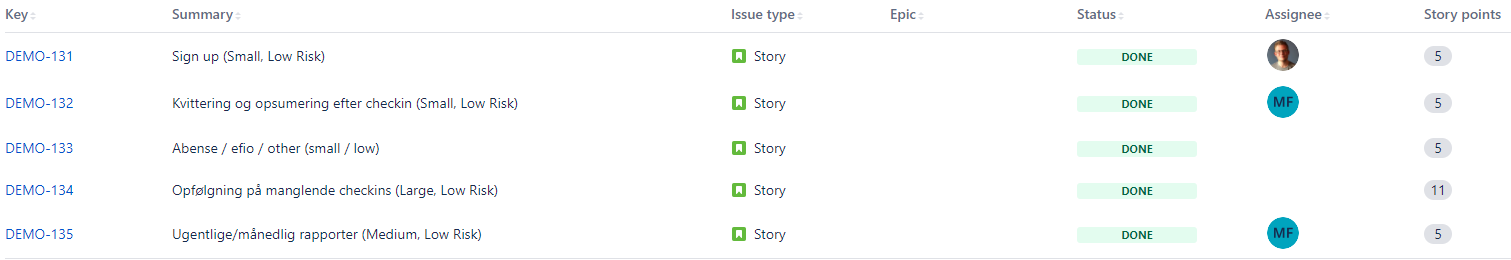
\includegraphics[height=4.13cm, width=15.92cm]{sprint5}
\end{center}

Jeg skulle opbygge en /command som brugere kunne benytte sig af til at registrere sig til systemet. 
Dette opnåede jeg ved opsætning af en lambdafunktion der trak alt identitetsinformation fra brugeren i Slack, 
og oprettede brugeren i databasen med et UUID, deres e-mail og deres Slack ID.

Herefter har jeg arbejdet på at få lavet en ugentlig rapport til brugeren, 
således at de kan få en oversigt over hvor mange timer de har været hos de forskellige kunder i den forrige uge. 
Her skulle databasen ændres således at der kom datoer på, så man havde mulighed for at kunne sortere efter datoerne. 
Herved var vi også nødt til at tjekke hvorvidt brugeren faktisk havde gennemført deres timeregistrering, hvis ikke det var 
udført blev det ikke talt med. Lambdafunktionen der får oprettet rapporten, 
har jeg sat op til at skulle køre hver eneste mandag kl. 9 om morgenen.

\chapter*{4. Refleksion}
\addcontentsline{toc}{chapter}{4. Refleksion}
Virksomheden har fået en slack applikation som de kan bruge til at indregistrere timer de har været hos kunder. 
Selv om systemet ikke er helt optimalt endnu, ligger der nu er godt fundament til systemet.

Praktikopholdet har været en stor fornøjelse med en god indsigt i hvordan man arbejder professionelt, 
hvordan man kommunikere og videregiver ens viden til hinanden på nemmeste måde. Alt vores kommunikation var igennem Slack, 
hvor vi kunne se hvordan de andre arbejdede sammen, samt hvordan vi havde kontakt med vores chef og gruppe. 

Jeg har lært utroligt meget nyt stof, serverless computing og opsættelse og brug af AWS. 
Det har været udfordrende at lære en masse nyt materiale som fungerer i nærheden af samme måde som det vi har lært i skolen. 
Men da man havde fået forståelsen for de forskellige produkter og services AWS har fungerer det utroligt godt sammen og 
kan nemt integreres med hinanden. Jeg regner selv med at bruge AWS til fremtidige projekter hvor der er mulighed for det.

At arbejde med scrum professionelt gav en helt anden oplevelse, ude hos Efio gav det overblik og var med til at skabe 
en klar proces for det arbejde man havde forude. Idét at scrum blev taget meget seriøst og at der var fokus på INVEST, 
planning poker og definition of done, gav det som helhed en virkelig god oplevelse og arbejdsgang. 
Hvor scrum på skolen mere har følt som noget man bare skulle få overstået og kørt igennem, 
kan jeg nu virkelig se værdierne i det som scrum giver til os som hold, og hvad det kan bidrage med. 

Jeg føler vi er kommet langt med vores produkt til Efio, og med alt hvad vi har lært og været igennem føler 
jeg mig godt rustet til at kunne begynde på hovedopgaven forude, som vi har haft muligheden for at kunne skrive på Efio.
 

\chapter*{5. Bilag}
\addcontentsline{toc}{chapter}{5. Bilag}
\section*{5.1 AWS Techical Professional Certification}
\addcontentsline{toc}{section}{5.1 AWS Techical Professional Certification}

\begin{center} 

\includegraphics[height=10.89cm, width=15.92cm]{aws-technical-professional}
\end{center}

\newpage

\section*{5.2 Efio's 4 kundesegmenter}
\addcontentsline{toc}{section}{5.2 Efio's 4 kundesegmenter}

\begin{center} 
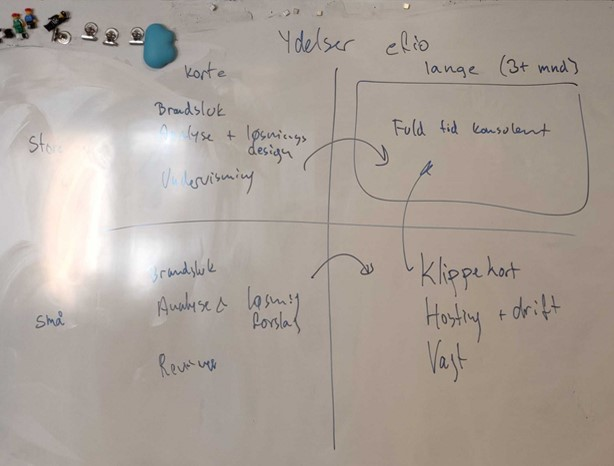
\includegraphics{kunde-segmenter}
\end{center}
Store virksomheder, kort ophold:
\begin{itemize}
  \item Brandsluk
  \item Analyse + løsningsdesign
  \item Undervisning
\end{itemize}
Små virksomheder, kort ophold:
\begin{itemize}
  \item Brandsluk
  \item Analyse + løsningsdesign
\end{itemize}
Store virksomheder, langt ophold:
\begin{itemize}
  \item Fuld tids konsulent
\end{itemize}
Små virksomheder, kort ophold:
\begin{itemize}
  \item Klippekort
  \item Hosting + drift
  \item Vagt
\end{itemize}

\newpage

\section*{5.3 Renskrevet backend arkitektur}
\addcontentsline{toc}{section}{5.3 Renskrevet backend arkitektur}
\begin{center} 
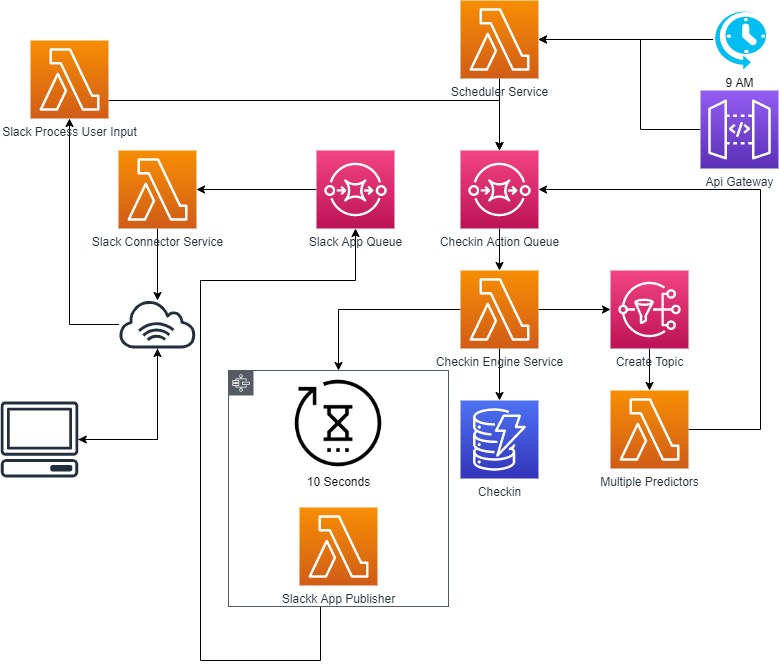
\includegraphics[height=12.39cm, width=15.92cm]{struktur-renskrevet}
\end{center}

\newpage

\section*{5.3 Systemet}
\addcontentsline{toc}{section}{5.3 Systemet}

\subsection*{Modal 1:}

\begin{center} 
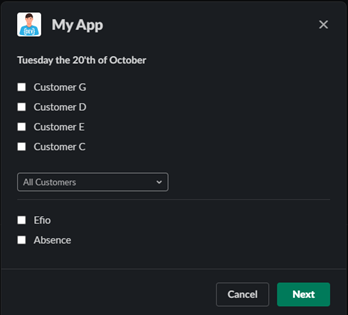
\includegraphics[height=8.35cm, width=9.2cm]{modal1}
\end{center}

\subsection*{Modal 2:}

\begin{center} 
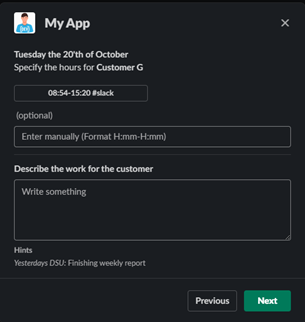
\includegraphics[height=8.35cm, width=9.2cm]{modal2}
\end{center}

\subsection*{Kvittering:}

\begin{center} 

\includegraphics[height=2.28cm, width=11.38cm]{kvittering}
\end{center}








\end{document}